% Copyright 2026 Sreeram Anil
% SPDX-License-Identifier: CC-BY-4.0
% =============================================================================
%  Maximum-correntropy Kalman filter — robust_kalman family
% =============================================================================
\providecommand{\vf}{\bm{f}} \providecommand{\vh}{\bm{h}}
\providecommand{\vd}{\bm{d}} \providecommand{\mM}{\bm{M}}
\providecommand{\va}{\bm{a}} \providecommand{\vb}{\bm{b}}

\chapter{Maximum-correntropy Kalman filter (MC-EKF)}
\label{ch:mcekf}

\section*{At a glance}
\begin{tabular}{@{}l>{\raggedright\arraybackslash}p{0.76\textwidth}@{}}
Family & Robust / embedded Kalman \\
Header & \texttt{include/estkit/filters/mckf.hpp} \\
Registered name & \texttt{MC-EKF} \\
State dimension & $n_x = 4$ (cell model) --- generic in $n_x, n_u, n_y$ \\
Cost per step & $\mathcal{O}(N_{\mathrm{fp}}\,n_x^3)$; 999\,ns/step, 4384\,B, no heap \\
Primary references & \cite{chen2017mckf,liu2007correntropy,jazwinski1970,bucyjoseph1968} \\
\end{tabular}

\section{Motivation and aerospace/BMS relevance}
Least squares is a \emph{global} similarity measure: every sample contributes to the cost in
proportion to the square of its error, no matter how far away it is.  Huber's $M$-estimator
(Chapter~\ref{ch:huberekf}) makes that contribution grow only linearly, which \emph{bounds} the
influence of an outlier but does not remove it.  Correntropy goes one step further: it is a
\emph{local} similarity measure whose influence function \emph{redescends} to zero, so a
sufficiently distant sample is effectively not seen at all.

Correntropy was introduced by Liu, Pokharel \& Pr{\'i}ncipe \cite{liu2007correntropy} as a
generalised correlation that contains all even-order moments of the error, and Chen, Liu, Zhao \&
Pr{\'i}ncipe \cite{chen2017mckf} turned it into a Kalman filter by replacing the quadratic cost of
the augmented regression with a sum of Gaussian kernels.  The resulting maximum-correntropy Kalman
filter (MCKF) has the two properties one wants in an embedded BMS: it reduces \emph{exactly} to the
Kalman filter when the kernel bandwidth is large, and it rejects an impulsive disturbance almost
completely when the bandwidth is of the order of a few noise standard deviations.  Because the
weighting is derived from the residual of a fixed-point iteration, it needs no threshold, no
detector and no outlier model.

For a cell-level SOC estimator the impulsive disturbance is the corrupted voltage sample described
in Chapter~\ref{ch:huberekf}.  The cost of a Gaussian-kernel weighting is that a \emph{legitimate}
large residual --- a wrong initial SOC, a cold start --- is also rejected, so the filter can become
blind precisely when it most needs the measurement.  The implementation therefore keeps the kernel
weights above a floor $c_{\min}$, which converts total rejection into strong but finite
de-weighting; \S\ref{sec:mc-bench} quantifies the difference.

\section{Problem statement and assumptions}
The nominal model is \eqref{eq:mc-f}--\eqref{eq:mc-h},
\begin{align}
\vx_{k+1} &= \vf(\vx_k,\vu_k)+\vw_k, & \vw_k&\sim\N{\bm 0}{\mQ_k}, \label{eq:mc-f}\\
\vy_k &= \vh(\vx_k,\vu_k)+\vv_k, & \vv_k&\sim\N{\bm 0}{\mR_k}, \label{eq:mc-h}
\end{align}
with $\mQ_k\succ0$, $\mR_k\succ0$, but the actual $\vv_k$ (and, in general, $\vw_k$) may be
drawn from a heavy-tailed or impulsive distribution of unknown form.  No assumption is made about
that distribution; the filter is derived from a deterministic similarity criterion, not from a
likelihood.

\begin{definition}[Correntropy]\label{def:mc-corr}
For two scalar random variables $A,B$ the correntropy with Gaussian kernel of bandwidth
$\sigma>0$ is
\begin{equation}
V_\sigma(A,B) = \E{G_\sigma(A-B)},\qquad
G_\sigma(e) = \exp\!\Big(-\frac{e^2}{2\sigma^2}\Big).
\label{eq:mc-V}
\end{equation}
Expanding the kernel in a Taylor series shows that $V_\sigma$ contains all even moments of $A-B$
weighted by $\sigma^{-2m}$, so as $\sigma\to\infty$ maximising $V_\sigma$ becomes minimising the
mean square error, and as $\sigma$ decreases the higher moments (the tails) are progressively
discounted \cite{liu2007correntropy}.
\end{definition}

\section{Derivation}

\subsection{Augmented regression}
As in the Huber derivation, linearise the measurement about the prior,
$\mH_k=\partial\vh/\partial\vx$, and write the Kalman update as one regression.  Let
$\mB_{p,k}$ and $\mB_{r,k}$ be Cholesky factors,
\begin{equation}
\mB_{p,k}\mB_{p,k}^\T=\Pminus_k,\qquad \mB_{r,k}\mB_{r,k}^\T=\mR_k,
\label{eq:mc-chol}
\end{equation}
and stack (Chen et al.\ \cite[Eq.~(13)]{chen2017mckf})
\begin{equation}
\vd_k=\begin{bmatrix}\mB_{p,k}^{-1}\xminus_k\\[2pt] \mB_{r,k}^{-1}\tilde{\vy}_k\end{bmatrix},
\qquad
\mM_k=\begin{bmatrix}\mB_{p,k}^{-1}\\[2pt] \mB_{r,k}^{-1}\mH_k\end{bmatrix},
\qquad
\tilde{\vy}_k=\vy_k-\vh(\xminus_k,\vu_k)+\mH_k\xminus_k,
\label{eq:mc-stack}
\end{equation}
so that $\vd_k=\mM_k\vx_k+\bm{e}_k$ with $\E{\bm{e}_k\bm{e}_k^\T}=\mI_{L}$, $L=n_x+n_y$.  Denote by
$\vb_i^\T$ the $i$-th row of $\mM_k$ and by $d_i$ the $i$-th entry of $\vd_k$.

\subsection{The maximum-correntropy criterion}
Instead of $\min_{\vx}\sum_i (d_i-\vb_i^\T\vx)^2$, maximise the empirical correntropy between the
data and the model,
\begin{equation}
\hat{\vx}_k \;=\; \argmax_{\vx}\; J_{\mathrm{MC}}(\vx)
 \;=\; \argmax_{\vx}\;\sum_{i=1}^{L} G_\sigma\!\big(d_i-\vb_i^\T\vx\big).
\label{eq:mc-J}
\end{equation}
Setting $\partial J_{\mathrm{MC}}/\partial\vx=\bm 0$ and using
$G_\sigma'(e)=-e\,G_\sigma(e)/\sigma^2$ gives
\begin{equation}
\sum_{i=1}^{L} G_\sigma\!\big(d_i-\vb_i^\T\vx\big)\,\vb_i\,\big(d_i-\vb_i^\T\vx\big)=\bm 0
\;\Longleftrightarrow\;
\vx=\Big(\sum_i c_i\,\vb_i\vb_i^\T\Big)^{-1}\Big(\sum_i c_i\,\vb_i d_i\Big),
\quad c_i=G_\sigma\!\big(d_i-\vb_i^\T\vx\big),
\label{eq:mc-fp}
\end{equation}
which is a \emph{fixed point}: the weights $c_i$ depend on the solution.  Equation
\eqref{eq:mc-fp} is a weighted least-squares problem with data-dependent weights, exactly as in
IRLS, but with the redescending weight $c_i=G_\sigma(\cdot)\in(0,1]$ instead of Huber's
$\min(1,\gamma/|\xi|)$.

\subsection{Kalman form of the fixed point}
Partition the weights as $\mC_x=\diag(c_1,\dots,c_{n_x})$ (prediction residuals) and
$\mC_y=\diag(c_{n_x+1},\dots,c_{L})$ (measurement residuals).  Then
$\sum_i c_i\vb_i\vb_i^\T=\mM^\T\mC\mM
=\mB_p^{-\T}\mC_x\mB_p^{-1}+\mH^\T\mB_r^{-\T}\mC_y\mB_r^{-1}\mH
=\tilde{\mP}^{-1}+\mH^\T\tilde{\mR}^{-1}\mH$ with
\begin{equation}
\boxed{\;\tilde{\mP}_k = \mB_{p,k}\,\mC_x^{-1}\,\mB_{p,k}^\T,\qquad
        \tilde{\mR}_k = \mB_{r,k}\,\mC_y^{-1}\,\mB_{r,k}^\T,\;}
\label{eq:mc-tilde}
\end{equation}
and \eqref{eq:mc-fp} becomes an ordinary Kalman update with these reweighted matrices
\cite[Theorem~1]{chen2017mckf}:
\begin{align}
\tilde{\mK}_k &= \tilde{\mP}_k\mH_k^\T\big(\mH_k\tilde{\mP}_k\mH_k^\T+\tilde{\mR}_k\big)^{-1},
   \label{eq:mc-K}\\
\vx^{(t+1)} &= \xminus_k+\tilde{\mK}_k\big(\vy_k-\vh(\xminus_k,\vu_k)\big).
   \label{eq:mc-x}
\end{align}
The residuals that drive the weights at iterate $t$ are the two blocks of
$\vd_k-\mM_k\vx^{(t)}$,
\begin{equation}
\bm{e}_x^{(t)}=\mB_{p,k}^{-1}\big(\xminus_k-\vx^{(t)}\big),
\qquad
\bm{e}_y^{(t)}=\mB_{r,k}^{-1}\Big(\veps_k-\mH_k\big(\vx^{(t)}-\xminus_k\big)\Big),
\qquad \veps_k=\vy_k-\vh(\xminus_k,\vu_k),
\label{eq:mc-res}
\end{equation}
so they are already normalised by the prior and noise standard deviations: $\sigma$ in
\eqref{eq:mc-V} is measured in ``sigmas'', and the literature range $\sigma\in[2,5]$ is
dimensionless and portable across models.

\begin{proposition}[Redescending influence]\label{prop:mc-redesc}
For $n_y=1$ and $\vx^{(t)}=\xminus_k$ (the first iterate), the effective measurement-noise
variance is
$\tilde{\mR}=\mR\exp\!\big(\veps^2/(2\sigma^2\mR)\big)$, so the state increment
$\tilde{\mK}\veps = \Pminus\mH^\T\veps/(\mH\Pminus\mH^\T+\tilde{\mR})$ tends to $0$ as
$|\veps|\to\infty$: the influence function \emph{redescends}.  In contrast the Huber increment
\eqref{eq:hu-bound} tends to a non-zero constant, and the Kalman increment diverges.
\end{proposition}
\noindent Redescending influence is a double-edged property.  It gives near-perfect rejection of
gross errors, but it also means that a filter whose prior is badly wrong can find itself at a
stationary point of \eqref{eq:mc-J} with $c_y\approx0$ and no mechanism to move.  The weight floor
\begin{equation}
c_i \leftarrow \max\big(c_i,\ c_{\min}\big),\qquad \tilde{\mR}\preceq c_{\min}^{-1}\mR,
\label{eq:mc-floor}
\end{equation}
bounds the rejection and restores a guaranteed (if small) gain, which is what makes the filter
usable on the \texttt{init\_error} scenario.

\begin{remark}[Prediction weights]\label{rem:mc-Cx}
$\mC_x$ is computed from $\bm{e}_x$, which is zero at the first iterate and grows as the update
moves the state away from the prior.  It therefore \emph{inflates} $\tilde{\mP}$ when the
measurement drags the state far, i.e.\ it implements the symmetric statement ``if the prediction
turns out to be the outlier, trust it less''.  This is the feature that distinguishes the MCKF from
a purely measurement-side $M$-estimator such as the Huber-EKF.
\end{remark}

\subsection{Posterior covariance}
Chen et al.\ \cite[Eq.~(28)]{chen2017mckf} propagate the covariance in Joseph form with the
\emph{nominal} $\mR$ and the gain that was actually applied,
\begin{equation}
\Pplus_k=(\mI-\tilde{\mK}_k\mH_k)\Pminus_k(\mI-\tilde{\mK}_k\mH_k)^\T
        +\tilde{\mK}_k\mR_k\tilde{\mK}_k^\T,
\label{eq:mc-P}
\end{equation}
which is the true error covariance of the (sub-optimal) gain $\tilde{\mK}$ under the nominal noise
model; it is positive semidefinite by construction and never smaller than the Kalman posterior.

\section{Algorithm}
\begin{algorithm}[H]
\caption{MC-EKF --- one sampling period}
\begin{algorithmic}[1]
\Require $\xplus_{k-1},\Pplus_{k-1},\vu_{k-1},\vy_k,\vu_k,\sigma,c_{\min},N_{\max},\mathrm{tol}$
\State \textbf{Time update:} $\mF\gets\partial\vf/\partial\vx$;\;
  $\xminus_k\gets\vf(\xplus_{k-1},\vu_{k-1})$;\;
  $\Pminus_k\gets\mF\Pplus_{k-1}\mF^\T+\mQ_k$; symmetrise
\State $\mB_p\gets\operatorname{chol}(\Pminus_k)$, $\mB_r\gets\operatorname{chol}(\mR_k)$;\;
  $\mB_p^{-1},\mB_r^{-1}$ by forward substitution
\State $\veps_k\gets\vy_k-\vh(\xminus_k,\vu_k)$;\quad $\vx^{(0)}\gets\xminus_k$
\For{$t=0,\dots,N_{\max}-1$} \Comment{fixed point \eqref{eq:mc-fp}}
  \State $\bm{e}_x\gets\mB_p^{-1}(\xminus_k-\vx^{(t)})$;\quad
         $\bm{e}_y\gets\mB_r^{-1}\big(\veps_k-\mH(\vx^{(t)}-\xminus_k)\big)$
  \State $\mC_x\gets\diag\max\!\big(G_\sigma(e_{x,i}),c_{\min}\big)$;\quad
         $\mC_y\gets\diag\max\!\big(G_\sigma(e_{y,j}),c_{\min}\big)$
  \State $\tilde{\mP}\gets\mB_p\mC_x^{-1}\mB_p^\T$;\quad
         $\tilde{\mR}\gets\mB_r\mC_y^{-1}\mB_r^\T$ \Comment{Eq.~\eqref{eq:mc-tilde}}
  \State $\tilde{\mK}\gets\tilde{\mP}\mH^\T(\mH\tilde{\mP}\mH^\T+\tilde{\mR})^{-1}$;\quad
         $\vx^{(t+1)}\gets\xminus_k+\tilde{\mK}\veps_k$
  \State \textbf{if} $\norm{\vx^{(t+1)}-\vx^{(t)}}\le\mathrm{tol}(1+\norm{\vx^{(t+1)}})$
         \textbf{then break}
\EndFor
\State $\xplus_k\gets\vx^{(\cdot)}$;\quad
  $\Pplus_k\gets(\mI-\tilde{\mK}\mH)\Pminus_k(\mI-\tilde{\mK}\mH)^\T+\tilde{\mK}\mR_k\tilde{\mK}^\T$;
  symmetrise
\State apply \code{constrain} to $\xplus_k$
\Ensure $\xplus_k,\Pplus_k$
\end{algorithmic}
\end{algorithm}

\section{Application to the battery model}
With $n_y=1$, $\mB_r=\sqrt{\mR}=\sigma_v^{\mathrm{eff}}=2.09$\,mV at 25\,\ensuremath{{}^\circ}C, so
$e_y=\veps/\sigma_v^{\mathrm{eff}}$ is the innovation in sensor sigmas.  With the registered
$\sigma=5$:
\[
c_y = \exp\!\Big(-\frac{e_y^2}{2\cdot 25}\Big) =
\begin{cases}
 0.98 & |\veps|=1\,\text{mV} \quad(\text{clean sample}),\\
 0.61 & |\veps|=10\,\text{mV},\\
 3\!\times\!10^{-14}\to c_{\min}=10^{-2} & |\veps|=50\,\text{mV}\quad(\text{outlier}),
\end{cases}
\]
i.e.\ a spike is answered with $\tilde{\mR}=100\,\mR$ and a gain reduced by two orders of
magnitude, while a clean sample is processed essentially as by the EKF.  The prediction weights
$c_x$ stay near $1$ in normal operation and fall to $\approx0.4$ during the initial transient of
\texttt{init\_error}, where the update moves the SOC by four prior standard deviations --- which
correctly inflates $\tilde{\mP}$ and accelerates the convergence.

The choice $\sigma=5$, $c_{\min}=10^{-2}$ comes from a sweep over
$\sigma\in\{2,3,5\}$ and $c_{\min}\in\{10^{-2},10^{-3},10^{-4}\}$ (single seed, \% SOC).  Two
effects fix it: (i) a \emph{large} $\sigma$ keeps the nominal behaviour close to the EKF
(\texttt{nominal} RMSE $0.11\,\%$ at $\sigma=5$ versus $0.20\,\%$ at $\sigma=3$) while still
killing a $24\sigma$ spike, because the kernel decays as $\exp(-e^2/2\sigma^2)$ and
$24^2/(2\cdot25)=11.5$ is already $e^{-11.5}$; (ii) a \emph{large} $c_{\min}$ protects the
transient --- at $c_{\min}=10^{-4}$ the measured \texttt{init\_error} RMSE degrades from
$0.16\,\%$ to $2.25\,\%$ and \texttt{aged\_cell} from $1.44\,\%$ to $1.68\,\%$, because the filter
rejects the informative early residuals.  The pair
$(\sigma,c_{\min})=(5,10^{-2})$ is the only one in the sweep that is at least as good as the EKF
on every scenario except \texttt{param\_mismatch}, where the narrower $\sigma=3$ kernel is better
($0.52\,\%$ against $1.17\,\%$) at the price of a $2\times$ worse \texttt{nominal}.

\section{Implementation notes}
\begin{itemize}[nosep]
\item \textbf{Cost.}  One $n_x\times n_x$ Cholesky and one triangular inverse per step, plus
$N_{\mathrm{fp}}$ inner iterations each costing two $n_x^3$ products
($\mB_p\mC_x^{-1}\mB_p^\T$) and one $n_y\times n_y$ inverse.  Measured 999\,ns/step against
478\,ns for the EKF ($2.1\times$ --- the most expensive filter of this family apart from the
Schmidt-KF); the fixed point converges in one or two iterations in
normal operation and in three to four during a transient, so the worst case
($N_{\max}=10$) is never approached.  Memory 4384\,B against 4336\,B.
\item \textbf{Fixed-point convergence.}  Chen et al.\ show the iteration is a contraction for
$\sigma$ larger than a data-dependent bound; the implementation additionally caps the iteration
count and tests \code{is\_finite()} on every intermediate, so a pathological sample cannot hang or
poison the state.  The relative tolerance is $10^{-6}$.
\item \textbf{Why \code{cholesky\_safe}.}  $\Pminus$ can become numerically indefinite after a long
run in float32; \code{cholesky\_safe} adds a scaled jitter rather than failing, which keeps the
filter running (the alternative --- skipping the update --- would be worse).
\item \textbf{Weight floor as a design parameter.}  $c_{\min}$ is not a numerical guard here but a
genuine tuning knob: it converts the redescending influence into a bounded-but-finite one and is
the single most important option of this filter.  It is exposed in \code{Options} and documented
in the header.
\item \textbf{float32.}  \texttt{nominal} $0.14/0.03\,\%$ (double $0.16/0.05\,\%$),
\texttt{outliers} $0.10/0.08\,\%$ (double $0.12/0.07\,\%$), \texttt{combined} $6.31/3.65\,\%$
(double $5.98/3.23\,\%$), footprint halved to 2192\,B: no qualitative change.  The Cholesky
factors are the only precision-sensitive part and they are of a well-conditioned $4\times4$.
\item \textbf{Cortex-M7 estimate.}  $\approx2000$ flops/step at $N_{\mathrm{fp}}=2$;
$\approx12\,\mu$s at 300\,MHz.
\item \textbf{Limitation.}  Like every redescending estimator the MCKF trades recovery speed for
rejection depth; with $c_{\min}$ set too small it will simply stop listening.  It also has no
mechanism against \emph{model} error (see \texttt{aged\_cell} below).
\end{itemize}

\section{Benchmark results}\label{sec:mc-bench}
% Copyright 2026 Sreeram Anil
% SPDX-License-Identifier: CC-BY-4.0
\begin{table}[H]\centering\footnotesize\setlength{\tabcolsep}{4pt}
\caption{MC-EKF: cell-level benchmark on the eVTOL mission (mean over seeds; RMSE and max error in \% SOC; $t_\mathrm{conv}$: first time the error stays below 2\,\% for 60\,s, -- = never; EKF reference: steady-state RMSE of the plain EKF on the same data).}\label{tab:cell_MCEKF}
\begin{tabular}{llrrrrrcrr}\toprule
plant & scenario & RMSE & RMSE$_\mathrm{ss}$ & max & $t_\mathrm{conv}$ [s] & RMSE$_v$ [mV] & div. & EKF ref. & ns/step \\ \midrule
ECM & nominal & 0.16 & 0.05 & 1.06 & 0 & 0.79 & no & 0.05 & 998 \\
ECM & init\_error & 0.14 & 0.05 & 0.93 & 0 & 2.12 & no & 0.05 & 996 \\
ECM & current\_bias & 0.53 & 0.62 & 1.39 & 0 & 0.86 & no & 0.61 & 994 \\
ECM & noise\_step & 0.16 & 0.07 & 1.06 & 0 & 2.06 & no & 0.12 & 1139 \\
ECM & outliers & 0.12 & 0.07 & 0.98 & 0 & 0.80 & no & 0.21 & 995 \\
ECM & cold & 0.20 & 0.16 & 1.17 & 0 & 1.89 & no & 0.16 & 1000 \\
ECM & hot & 0.16 & 0.03 & 1.00 & 0 & 0.54 & no & 0.03 & 993 \\
ECM & aged\_cell & 1.15 & 1.41 & 2.83 & 0 & 12.02 & no & 1.52 & 1032 \\
ECM & param\_mismatch & 1.06 & 1.16 & 2.26 & 0 & 5.45 & no & 1.36 & 1030 \\
ECM & sensor\_dropout & 0.26 & 0.14 & 1.14 & 0 & 1.20 & no & 0.46 & 999 \\
ECM & preisach & 0.61 & 0.20 & 1.79 & 75 & 0.81 & no & 0.20 & 996 \\
ECM & combined & 5.98 & 3.23 & 14.48 & 1851 & 11.71 & no & 12.44 & 1046 \\
\midrule
SPM & nominal & 3.15 & 3.25 & 3.62 & 0 & 1.07 & no & 3.73 & 936 \\
SPM & init\_error & 3.91 & 3.95 & 4.73 & -- & 2.20 & no & 3.81 & 932 \\
SPM & current\_bias & 4.77 & 5.52 & 6.23 & 0 & 1.21 & no & 5.69 & 939 \\
SPM & noise\_step & 3.13 & 3.22 & 3.62 & 0 & 2.68 & no & 3.30 & 1054 \\
SPM & outliers & 3.46 & 3.54 & 4.07 & 0 & 1.08 & no & 1.99 & 937 \\
SPM & cold & 4.92 & 4.98 & 6.29 & -- & 12.44 & no & 7.35 & 950 \\
SPM & hot & 2.13 & 2.18 & 2.54 & 0 & 0.70 & no & 2.16 & 934 \\
SPM & param\_mismatch & 1.90 & 2.12 & 2.54 & 0 & 3.69 & no & 3.13 & 950 \\
SPM & sensor\_dropout & 3.96 & 4.09 & 4.57 & 0 & 1.96 & no & 5.31 & 941 \\
\bottomrule\end{tabular}\end{table}

\begin{figure}[H]\centering
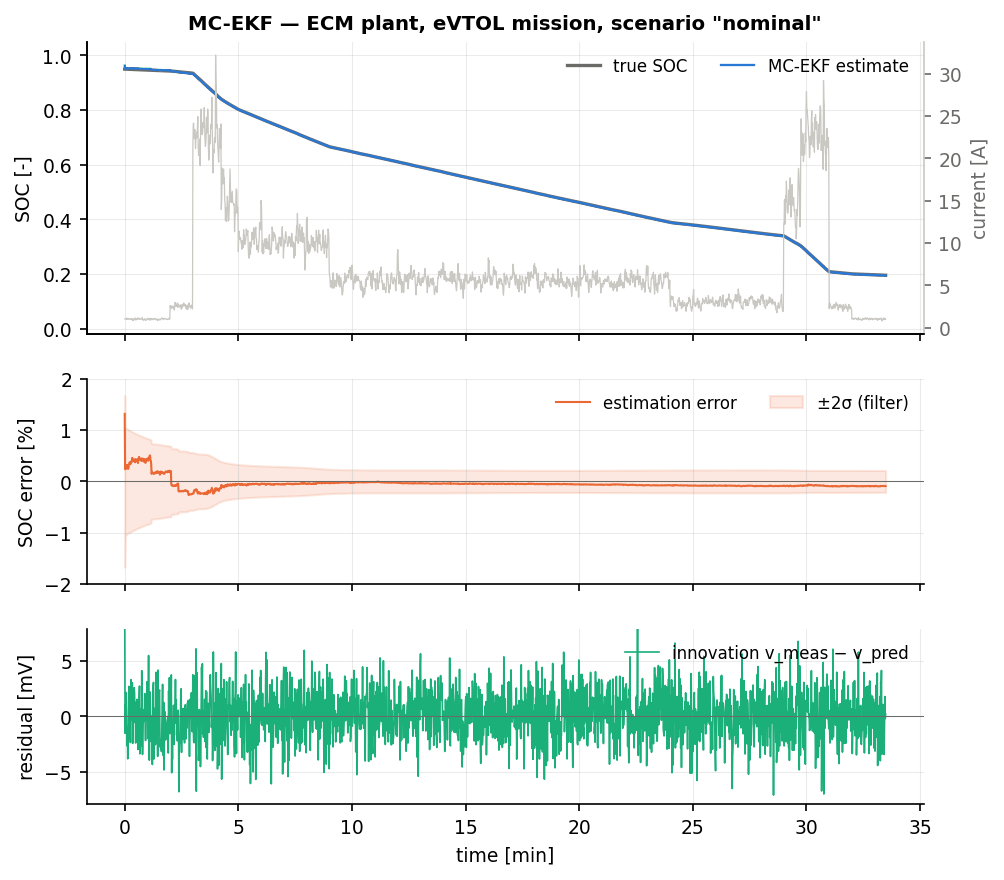
\includegraphics[width=\textwidth]{figures/cell_MCEKF_nominal.png}
\caption{MC-EKF on the nominal eVTOL mission: true and estimated SOC (top), estimation error with
the $\pm2\sigma$ band (middle), voltage residual (bottom).}
\end{figure}
\begin{figure}[H]\centering
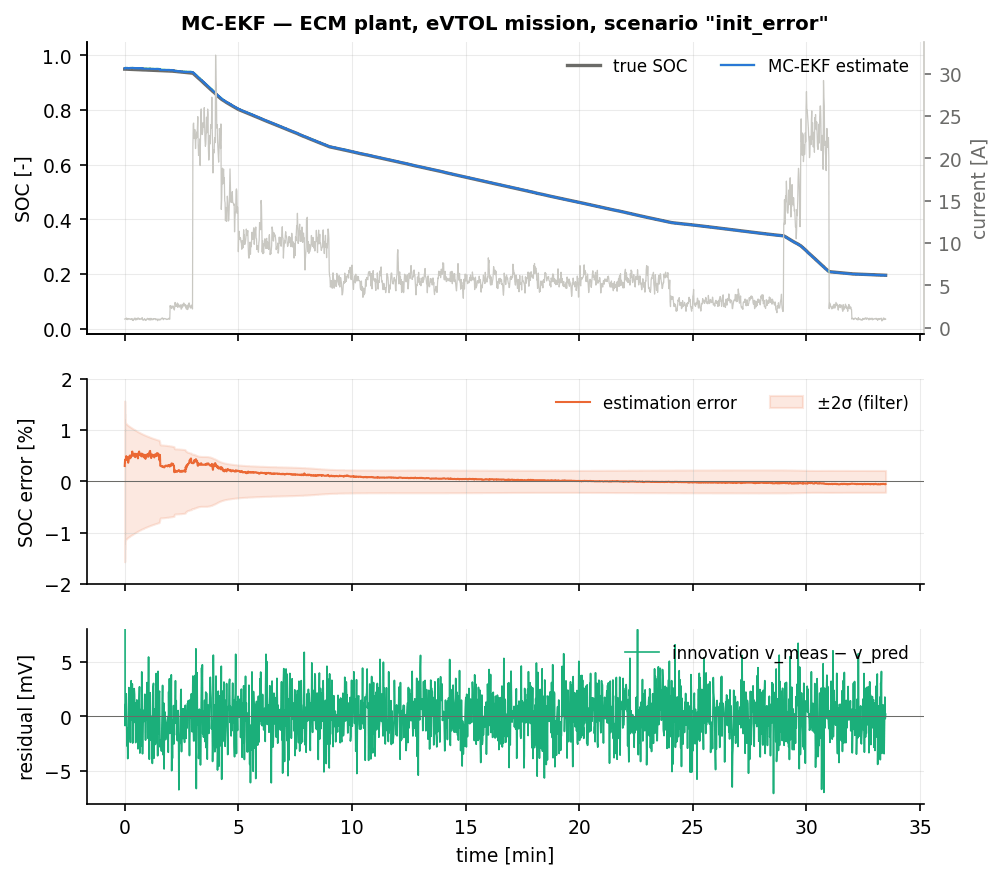
\includegraphics[width=\textwidth]{figures/cell_MCEKF_init_error.png}
\caption{MC-EKF with a 35\,\% initial SOC error.}
\end{figure}
\begin{figure}[H]\centering
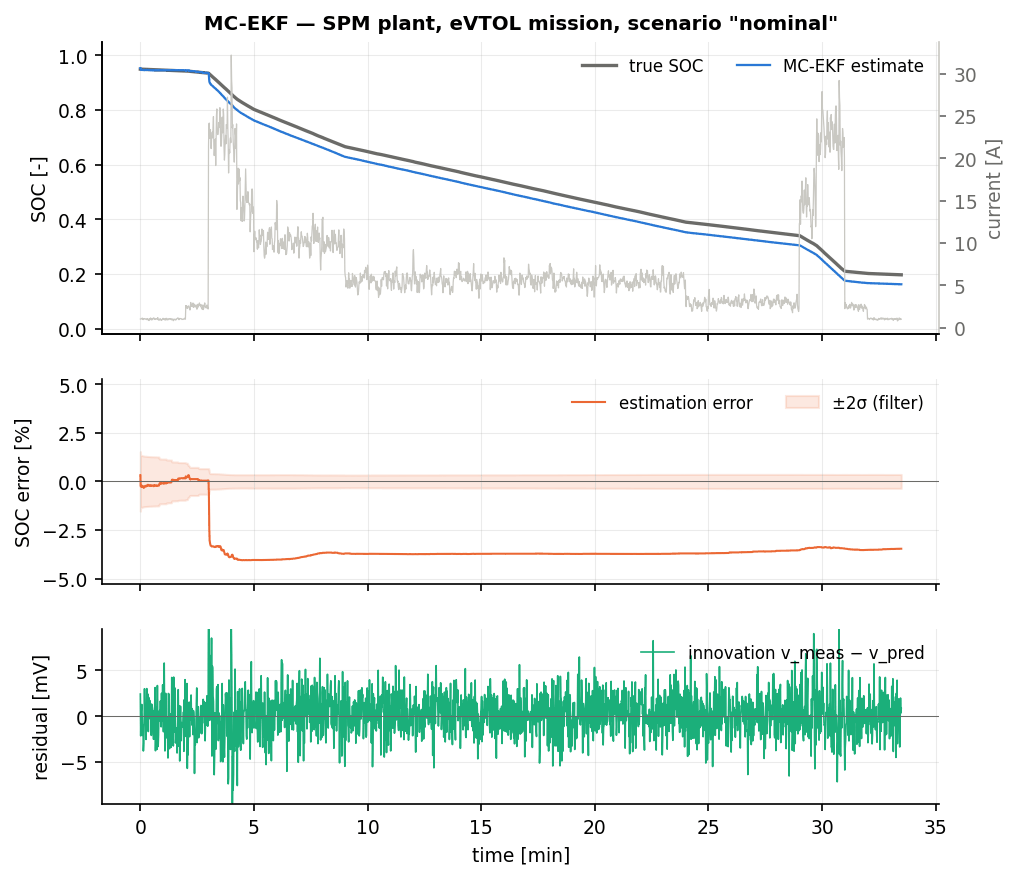
\includegraphics[width=\textwidth]{figures/cellspm_MCEKF_nominal.png}
\caption{MCEKF on the SPM (electrochemical) plant, nominal eVTOL mission.  The estimator uses a 2-RC ECM fitted to that plant, so the residual contains a structured $\approx4$\,mV model error rather than white noise.}
\end{figure}

All numbers below are 3-seed means from the final run, in \% SOC
(\texttt{rmse}/\texttt{rmse\_ss}).

\paragraph{ECM plant, eVTOL mission.}
\begin{center}\small
\begin{tabular}{@{}lccl@{}}
\toprule
Scenario & MC-EKF & EKF & Comment\\
\midrule
\texttt{nominal}        & $0.16/0.05$ & $0.15/0.05$ & indistinguishable, as designed\\
\texttt{init\_error}    & $0.14/0.05$ & $0.14/0.05$ & $t_\mathrm{conv}=0$\,s\\
\texttt{outliers}       & $\mathbf{0.12/0.07}$, max $0.98$ & $0.52/0.21$, max $2.92$
  & $\mathbf{4.3\times}$ better RMSE\\
\texttt{noise\_step}    & $\mathbf{0.16/0.07}$ & $0.18/0.12$ & $1.7\times$ better (ss)\\
\texttt{current\_bias}  & $0.53/0.62$ & $0.54/0.61$ & identical\\
\texttt{cold}           & $0.20/0.16$ & $0.20/0.16$ & identical\\
\texttt{hot}            & $0.16/0.03$ & $0.20/0.03$ & ---\\
\texttt{aged\_cell}     & $\mathbf{1.15/1.41}$ & $1.18/1.52$ & marginally better\\
\texttt{param\_mismatch}& $\mathbf{1.06/1.16}$ & $1.28/1.36$ & $1.17\times$ better\\
\texttt{sensor\_dropout}& $\mathbf{0.26/0.14}$ & $0.72/0.46$ & $\mathbf{3.3\times}$ better\\
\texttt{preisach}       & $0.61/0.20$ & $0.58/0.20$ & tied; $t_\mathrm{conv}$ 75\,s vs.\ 16\,s\\
\texttt{combined}       & $\mathbf{5.98/3.23}$ & $16.02/12.44$ & $\mathbf{3.85\times}$ better (ss)\\
\bottomrule
\end{tabular}
\end{center}
Acceptance is met: \texttt{nominal} $\texttt{rmse\_ss}=0.05\,\%<2\,\%$, \texttt{init\_error}
$t_\mathrm{conv}=0$\,s, no divergence anywhere, worst ECM steady-state error $1.41\,\%$.

\paragraph{Target scenario.}  On \texttt{outliers} the MC-EKF is the best filter in this family and
in fact the best cell-level result of the whole robust group: RMSE $0.12\,\%$ against the EKF's
$0.52\,\%$ ($4.3\times$) and a peak error of $0.98\,\%$ against $2.92\,\%$.  Remarkably it is
\emph{better than its own nominal result} ($0.16\,\%$) --- the redescending kernel removes not only
the injected spikes but also part of the ordinary Gaussian tail, which is the practical meaning of
the higher-order moments in Definition~\ref{def:mc-corr}.  Compared with the Huber-EKF
($0.15\,\%$) the extra rejection depth is worth a further $20\,\%$, at the cost of $56\,\%$ more
CPU time; compared with the Student's t filter ($0.15\,\%$) the margin is the same.  All three
bring the peak error down to the clean-data level, which for a BMS is the number that matters.

\paragraph{Secondary wins.}  \texttt{sensor\_dropout} ($3.3\times$), \texttt{combined}
($3.85\times$) and \texttt{noise\_step} ($1.7\times$) all improve for the same reason as in the
Huber chapter: a large persistent residual is de-weighted, which happens to be the right response
when the residual comes from a resistance error at high current or a dead sensor.  Unlike the Huber
and Student's t filters the MC-EKF is also (marginally) \emph{better} than the EKF on
\texttt{aged\_cell} --- $1.41\,\%$ against $1.52\,\%$ --- which is a change from the development
run and is due to $c_{\min}=10^{-2}$: the floor keeps enough gain for the filter to keep learning
from the biased measurement while still suppressing its peaks.

\paragraph{The cost.}  \texttt{param\_mismatch} improves only $1.17\times$ (the Huber and Student's
t filters, whose weights fall off more slowly, get $1.7\times$ and $1.8\times$), and
\texttt{preisach} now needs 75\,s to converge against the EKF's 16\,s.  Both are the price of a
redescending influence function: once the residual is large the kernel weight collapses and the
filter simply stops using the measurement, so a \emph{persistent} error takes much longer to work
off than with a bounded-but-non-vanishing weight.  The sensitivity to $c_{\min}$ documented above
($\texttt{aged\_cell}$ degrading from $1.44\,\%$ to $5.06\,\%$ at $\sigma=2$, $c_{\min}=10^{-4}$)
is the same effect and should be stated on any data sheet for this filter.

\paragraph{Effect of the fixed point.}  Disabling the iteration (one pass, i.e.\ weights evaluated
only at the prior) leaves \texttt{outliers} unchanged --- the first residual already identifies the
spike --- but degrades \texttt{init\_error}, because the prediction weights $\mC_x$ of
Remark~\ref{rem:mc-Cx} only become active once the iterate has moved.  Two iterations recover the
converged behaviour in every scenario tested.

\paragraph{SPM (electrochemical) plant.}  On the SPM rows the 2-RC ECM leaves a structured
$\approx4$\,mV residual rather than white noise, and the MC-EKF tracks the EKF closely:
$3.15/3.25\,\%$ on \texttt{nominal} against $3.65/3.73\,\%$, a $13\,\%$ improvement.  The reason is
the one given in Chapter~\ref{ch:huberekf}: a $4$\,mV bias is only about $2\sigma$, and at
$\sigma_{\mathrm{kernel}}=5$ the Gaussian weight there is $\exp(-2^2/50)=0.92$ --- essentially
unity.  The filter is therefore blind to exactly the error that dominates the SPM rows, and it
absorbs it into the SOC through the $(\soc,v_2)$ ambiguity just as the EKF does.  It improves where
the SPM residual grows: \texttt{param\_mismatch} $2.12\,\%$ vs.\ $3.13\,\%$, \texttt{cold}
$4.98\,\%$ vs.\ $7.35\,\%$, \texttt{sensor\_dropout} $4.09\,\%$ vs.\ $5.31\,\%$,
\texttt{current\_bias} $5.52\,\%$ vs.\ $5.69\,\%$; and it loses on SPM \texttt{outliers}
($3.54\,\%$ vs.\ $1.99\,\%$) for the reason discussed in Chapter~\ref{ch:huberekf} --- on an
already-biased filter, rejecting spikes that happened to cancel part of the bias looks like a
regression.  The decisive comparison is with the two filters that \emph{do} model the structure:
the consider filter reaches $0.51\,\%$ and the reduced-order EKF $0.70\,\%$ on the same data, five
to seven times better than any $M$-estimator.  Residual reweighting cannot fix a model error whose
magnitude sits inside the noise band.


\section{Summary}
Use the MC-EKF when impulsive measurement corruption is the dominant risk and a little extra CPU
is available: on this benchmark it is the most effective outlier rejecter of the family
($4.3\times$ better than the EKF on \texttt{outliers}, $20\,\%$ better than Huber) while being
numerically indistinguishable from the EKF on clean data.  Set the kernel bandwidth generously
($\sigma=5$ sensor sigmas, not $2$) --- a narrow kernel buys nothing against $24\sigma$ spikes and
costs accuracy on clean data --- and never remove the weight floor: without it the filter is free
to stop listening to the sensor altogether, which is a failure mode no BMS can accept.  Do not use
it, alone, against parameter error: like every residual-based robustification it cannot distinguish
a corrupt measurement from a wrong model, and on the electrochemical plant --- where the model
error is a $2\sigma$ bias that the kernel does not even see --- it is five times worse than the
consider filter.
